\documentclass[12pt]{article}
\usepackage[margin=0.7in]{geometry}
\usepackage{graphicx}
\usepackage{float}
\usepackage{amsmath}

\begin{document}

\begin{titlepage}

\newcommand{\HRule}{\rule{\linewidth}{0.5mm}} % Defines a new command for the horizontal lines, change thickness here

\center % Center everything on the page

%----------------------------------------------------------------------------------------
%	HEADING SECTIONS
%----------------------------------------------------------------------------------------

\textsc{\LARGE Drexel University}\\[1.5cm] % Name of your university/college
\textsc{\Large CS499I}\\[0.5cm] % Major heading such as course name
\textsc{\large Advanced Neural Networks}\\[0.5cm] % Minor heading such as course title

%----------------------------------------------------------------------------------------
%	TITLE SECTION
%----------------------------------------------------------------------------------------

\HRule \\[0.4cm]
{ \huge \bfseries Facial Recognition With Artificial Neural Networks}\\[0.4cm] % Title of your document
\HRule \\[1.5cm]

%----------------------------------------------------------------------------------------
%	AUTHOR SECTION
%----------------------------------------------------------------------------------------

\begin{minipage}{0.4\textwidth}
\begin{flushleft} \large
\emph{Author:}\\
Alexander \textsc{Marion}\\
Matthew \textsc{D'Amore}
\end{flushleft}
\end{minipage}
~
\begin{minipage}{0.4\textwidth}
\begin{flushright} \large
\emph{Supervisor:} \\
Dr. Matthew \textsc{Burlick}
\end{flushright}
\end{minipage}\\[4cm]

% If you don't want a supervisor, uncomment the two lines below and remove the section above
%\Large \emph{Author:}\\
%John \textsc{Smith}\\[3cm] % Your name

%----------------------------------------------------------------------------------------
%	DATE SECTION
%----------------------------------------------------------------------------------------

{\large \today}\\[3cm] % Date, change the \today to a set date if you want to be precise

%----------------------------------------------------------------------------------------
%	LOGO SECTION
%----------------------------------------------------------------------------------------

%\includegraphics{Logo}\\[1cm] % Include a department/university logo - this will require the graphicx package

%----------------------------------------------------------------------------------------

\vfill % Fill the rest of the page with whitespace
\end{titlepage}

\newpage

\section{Datasets}
\textbf{Yale Faces Database} \quad This dataset contains 165 grayscale images in GIF format of 15 individuals with 11 images per person. There is one image per each of the following configurations: center-light, w/glasses, happy, left-light, w/no glasses, normal, right-light, sad, sleepy, surprised, and wink.

\section{Testing Parameters}
The following variants are tested for accuracy:
\begin{enumerate}
  \item With and without a bias node at the input layer
  \item With and without a bias node at the hidden layer
  \item With and without standardizing features
  \item With and without applying PCA to reduce the number of features to 95\%
  \item With and without applying LDA to maximize data separability
\end{enumerate}
Empirical data was generated to optimize the following parameters:
\begin{enumerate}
  \item Image size
  \item Hidden layer size
  \item Termination criteria
\end{enumerate}

\section{Baseline Accuracy}
The baseline accuracy was created using the negative form of all variants with the exception of data standardization. Initial parameters are listed below:
\begin{enumerate}
  \item Input layer bias node: N
  \item Hidden layer bias node: N
  \item Standardization of features: Y
  \item PCA application: N
  \item LDA application: N
  \item Image size: 40x40
  \item Hidden layer size: 20
  \item Termination criteria: 1000 iterations
\end{enumerate}
\begin{table}[h]
  \begin{center}
    \begin{tabular}{|l|l|}
      \hline
      Accuracy & 0.800000\\
      Testing Error & 0.200000\\
      \hline
    \end{tabular}
    \caption{ANN Testing Error}
  \end{center}
\end{table}

\section{Artificial Neural Networks}
\begin{table}[h]
\begin{center}
\begin{tabular}{|l|l|}
\hline
Accuracy & 0.940639\\
Testing Error & 0.059361\\
\hline
\end{tabular}
\caption{ANN Testing Error}
\end{center}
\end{table}


\begin{figure}[H]
\begin{center}
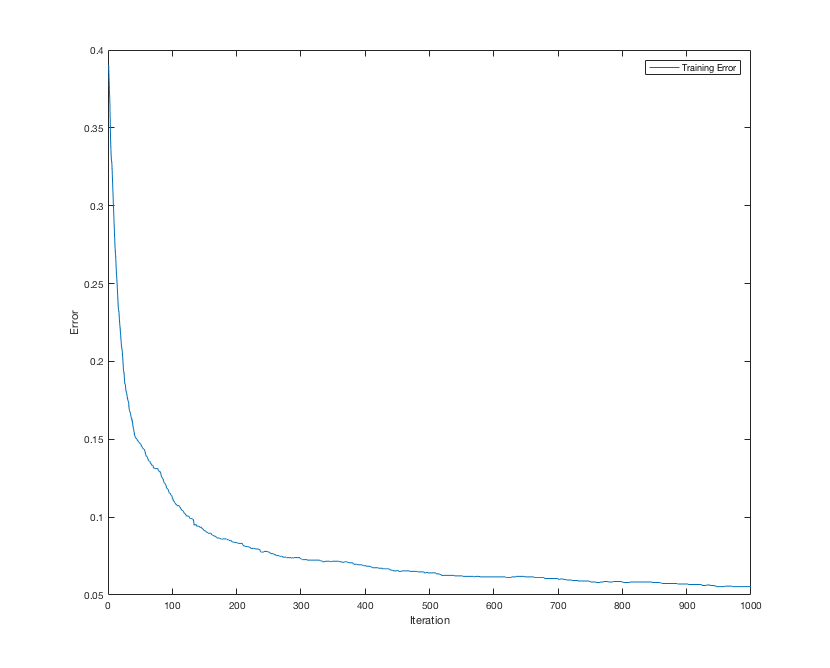
\includegraphics[height=11cm]{problem1_training_error.png}
\caption{Training Error for ANN}
\end{center}
\end{figure}

\newpage

\section{The Precision-Recall Tradeoff}\label{naive}
\begin{figure}[H]
\begin{center}
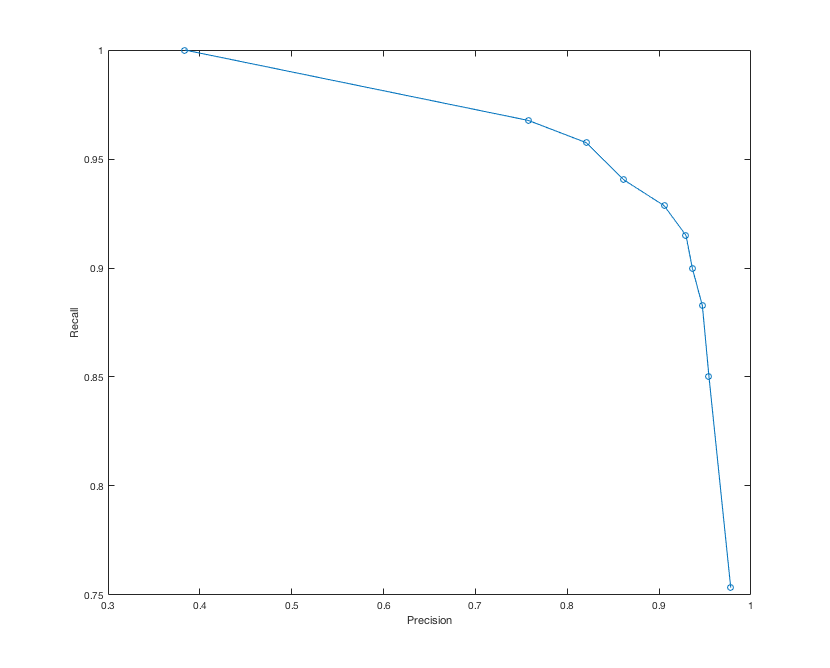
\includegraphics[height=11cm]{problem2_PRC.png}
\caption{PR-Graph for ANN}
\end{center}
\end{figure}

\newpage
\section{Multi-Class Artificial Neural Networks}
\begin{table}[h]
\begin{center}
\begin{tabular}{|l|l|}
\hline
Accuracy & 0.956215\\
Testing Error & 0.043785\\
\hline
\end{tabular}
\caption{ANN Testing Error}
\end{center}
\end{table}

\begin{figure}[H]
\begin{center}
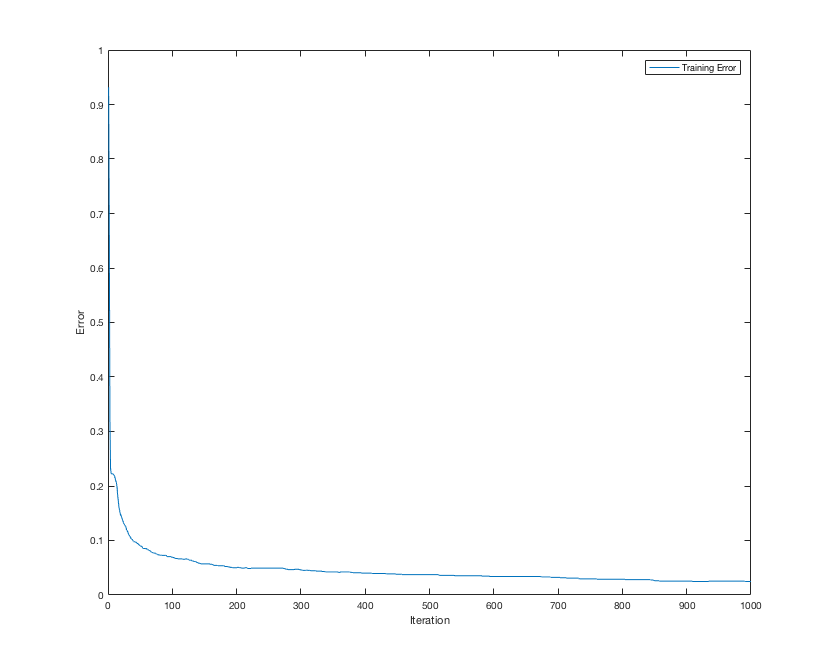
\includegraphics[height=11cm]{problem3_training_error.png}
\caption{Training Error for Multi-Class ANN}
\end{center}
\end{figure}
\end{document}
